\section{Test de Kolmogorov-Smirnov}
\subsection{Test de Kolmogorov-Smirnov para hipótesis simples}

$X_1,\dots, X_n$ i.i.d. con función de distribución F continua y se quiere contrastar
\[
    H_0: F=F_0 \quad H_1: F \neq F_0
\]

El test de Kolmogorov-Smirnov es más potente que el $\chi^2$ en el caso de F continua.
Tenemos:
\begin{itemize}
    \item $F_0 \to $ Función de distribusión bajo $H_0$.
    \item $\widehat{F_n} \to$ Función de distribución muestral o empírica.
\end{itemize}
\[
    \widehat{F_n}(x)=\frac{1}{n} \sum_{i=1}^{n} \mathbbm{1}_{(x_i \leq x)}, \quad x \in \mathrm{R}
\]
Tambien se puede definir a partir de los estadísticos de orden:

\[
    \widehat{F_n}(x)=
    \left\{
    \begin{array}{ll}
        0, & \text{si} \quad x \leq X_{(1)}\\
        \frac{i}{n} & \text{si} \quad X_{(i)} \leq x \leq X_{(i+1)}, \quad i=1, \dots,n-1 \\
        1 & \text{si} \quad X_n \leq x
    \end{array}
    \right.
\]

Propiedades:
\begin{enumerate}
    \item $n\cdot \widehat{F_n}(x)$ es el total de valores de la muestra menores o iguales a $x$y sigue una distribución $B(n, F(x))$, $\forall x \in \mathbb{R}$
    \item Según el resultado anterior, junto con las propiedades de la distribución binomial, se tiene $\widehat{F}$(x) es un estimador consistente de $F(x)$
    \[
        \lim_{n \to \infty} P(|\widehat{F_n}(x) - F(x)| < \varepsilon) \to 0
    \]
    \[
        \text{y es CAN: }\sqrt{n}\cdot(\widehat{F_n}(x)-F(x))\backsimeq N(0,F(x)(1-F(x)))
    \]
    \item Por el teorema de Glivenko-Cantelli, $\widehat{F_n}(x)$ converge uniformemente y casi seguro a $F(x)$.
\end{enumerate}

A medida que n crece, al función escalonada de $\widehat{F_n}(x)$ con saltos en los valores de los estadísticos de orden $X_{(1)},\dots,X_{(n)}$ aproxima la distribución $F(x)'$.  % Creo que eso no debería ser prima pero no soy un experto

Por lo tanto cuando n es grande, la mayor diferencia entre $\widehat{F_n}(x)$ y $F(x)$ converge a 0.

Este resultado nos sugiere el estadístico $D_n=sup_x[\widehat{F_n}(x)-F(x)]$ el cual es una medida razonable de la precisión de la estimación.

Llamaremos estadístico de Kolmogorov-Smirnov de una muestra a
\[
    D_n=sup_x|\widehat{F_n}(x)-F_0(x)|
\]
El test rechaza la hipótesis para valores grandes del estadísitico ($D_n>C$).
Como siempre debemos conocer la distribución de $D_n$ para obtener el valor crítico.

\begin{enumerate}
    \item Es importante ver que la máxima diferencia en $|\widehat{F_n}(x)-F_0(x)|$ es la máxima 
    diferencia en los puntos en los que $\widehat{F_n}(x)>F_0(x)$ y la máxima en los punto donde $F_0(x)>\widehat{F_n}(x)$. 
    Así podemos definir los estadísticos Kolmogorov-Smirnov de un lado.
    \[
        \left.\begin{matrix}
                D_n^+=sup_x(\widehat{F_n}(x)-F_0(x)) \\
                D_n^-=sup_x(F_0(x)-\widetilde{F_n}(x))
        \end{matrix}\right\}
        D_n=max\{D_n^+,D_n^-\}
    \]
            
    $D_n^+$ y $D_n^-$ son útiles para conocer la distribución.

    \item La distribución de $D_n^+$, $D_n^-$ y $D_n$ no depende de $F_0$, es decir, $c_\alpha$ será el mismo sin importar si estamos contrastando diferentes hipótesis simples (Como por ejemplo $N(3,1)$, $exp(2)$, $\dots$). Se dice que el estadístivo es de distribución libre ya que no depende de $F_0$.
\end{enumerate}

\begin{figure}[h!]
    \centering
    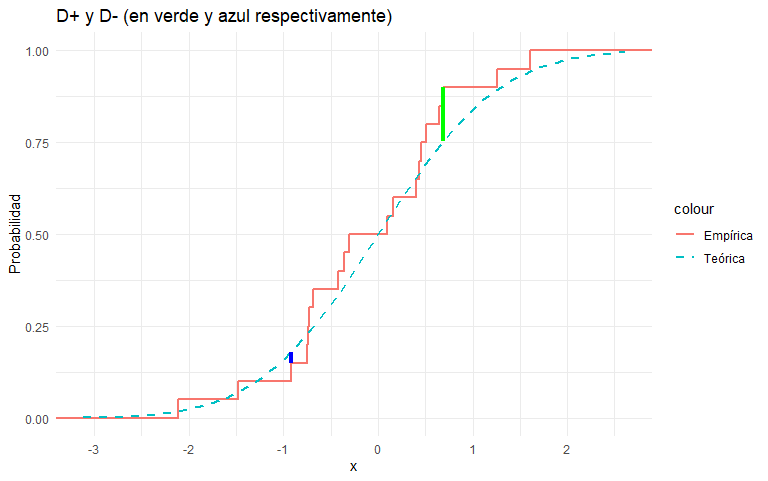
\includegraphics[width=\textwidth]{assets/EjemploD.png}
    \caption{Visualización del estadísitico D+ y D-}
    \label{fig:Dplus_Dminus}
\end{figure}

Definimos los estadísticos de orden como $X_{(0)}=-\infty$ y $X_{(n)}=+\infty$, por lo tanto podemos definir $\widehat{F_n}(x)=\frac{i}{n} \quad \forall X_{(i)} \leq x < X_{(i+1)}$.

$D_n^+$ lo podemos ir calculando a trozos como:

\[
    D_n^+=sup_x(\widehat{F_n}(x)-F_0(x))
\]
    
Tomará un valor máximo unicamente en los extremos del intervalo $[X_{(i)},X_{(i+1)})$        
            
\[
    D_n^+=max_{1 \leq i \leq n}\left(\frac{i}{n}-F_0(x_{(i)})\right)
\]
Análogamente:
\[
    D_n^-=max_{1 \leq i \leq n}\left(F_0(x_{(i)})-\frac{i-1}{n}\right)
\]
$D_n^+,D_n^-$(por lo tanto $D_n$) dependen de las variables aleatorias.
\[
F_0(X_{(1)}),\dots,F_0(X_{(n)}) \sim U(0,1)
\]
Esto ocurre por la trasnformada integral de probabilidad, siempre y cuando las variables aleatorias sean continuas.

\subsection{Test de Kolmogorov-Smirnov para una hipótesis compuesta}

Lo anterior nos sirve para hipótesis simp,es. Sin embargo en la mayoría de los escenarios reales, tenemos hipótesis compuestas.
Por ejemplo, utlizar Kolmogorov-Smirnov en ANOVA.

Situación:
\[
H_0: F=F_0(\theta) \quad H_1:F \neq F_0(\theta)
\]
Lo haremos como siempre:
\begin{enumerate}
    \item Estimamos $\theta$ a partir de los datos(con el Estimador Máximo Verosimil).
    \item Se calcula el estadístico Kolmogorov-Smirnov como en el caso de la hipótesis simple:
    \[
    \widehat{D_n}=sup_\chi|\widehat{F_n}(\chi)-F(\chi)|
    \]
    Se rechaza $H_0$ con valores grandes de $\widehat{D_n}$ ($\widehat{D_n}>C$). 
    
    Es importante recalcar que $\widehat{D_n}$ no sigue la misma distribución que $D_n$.
    La distribución no es libre, depende de la familia que estemos evaluando.
\end{enumerate}

Tenemos tablas obtenidas por \href{https://es.wikipedia.org/wiki/Prueba_de_Lilliefors}{Lilliefors}
por simulación para la normal y para la exponencial.
Pasos a seguir:
\begin{enumerate}
    \item Se estiman los parámetros $\hat{\mu}$ y $\widehat{\lambda}$
    \item Se obtiene la muestra estandarizada $z_1,\dots,z_n$.
    \item Hacer el test ($H_0:F_0 \equiv N(0,1)$ en el caso normal y $H_0:F_0\equiv exp(1)$ en el caso exponencial).
    \item Se rechaza $H_0$ si $\widehat{D_n}>C$ para nivel $\alpha$. Se usan las tablas de \href{https://es.wikipedia.org/wiki/Prueba_de_Lilliefors}{Lilliefors}
    para definir $C_\alpha$.
\end{enumerate}

\subsubsection*{Caso exponencial:}

\[
\begin{matrix}
    H_0:F \equiv exp(\lambda) \\
    H_1:F \neq exp(\lambda)
\end{matrix}
\]
\[
    \widehat{\lambda}=\frac{1}{\bar{X}}, \quad z_i
    =\frac{X_i}{\bar{X}} \to z_i \sim exp(1) \longrightarrow\gamma(1,\lambda)
\]
El contraste es equivalente a:
\[
    H_0: X \sim \gamma\left(1,\frac{1}{\bar{X}}\right) \longleftrightarrow H_0:Z \sim \gamma(1,1)
\]

Podrás descubrir más estadísticos en el campus virtual
